\documentclass[letterpaper, 11pt]{extarticle}
% \usepackage{fontspec}

% ==================================================

% document parameters
% \usepackage[spanish, mexico, es-lcroman]{babel}
\usepackage[english]{babel}
\usepackage[margin = 1in]{geometry}

% ==================================================

% Packages for math
\usepackage{mathrsfs}
\usepackage{amsfonts}
\usepackage{amsmath}
\usepackage{amsthm}
\usepackage{amssymb}
\usepackage{physics}
\usepackage{dsfont}
\usepackage{esint}

% ==================================================

% Packages for writing
\usepackage{enumerate}
\usepackage[shortlabels]{enumitem}
\usepackage{framed}
\usepackage{csquotes}

% ==================================================

% Miscellaneous packages
\usepackage{float}
\usepackage{tabularx}
\usepackage{xcolor}
\usepackage{multicol}
\usepackage{subcaption}
\usepackage{caption}
\captionsetup{format = hang, margin = 10pt, font = small, labelfont = bf}

% Citation
\usepackage[round, authoryear]{natbib}

% Hyperlinks setup
\usepackage{hyperref}
\definecolor{links}{rgb}{0.36,0.54,0.66}
\hypersetup{
   colorlinks = true,
    linkcolor = black,
     urlcolor = blue,
    citecolor = blue,
    filecolor = blue,
    pdfauthor = {Author},
     pdftitle = {Title},
   pdfsubject = {subject},
  pdfkeywords = {one, two},
  pdfproducer = {LaTeX},
   pdfcreator = {pdfLaTeX},
   }
\usepackage{titlesec}
\usepackage[many]{tcolorbox}

% Adjust spacing after the chapter title
\titlespacing*{\chapter}{0cm}{-2.0cm}{0.50cm}
\titlespacing*{\section}{0cm}{0.50cm}{0.25cm}

% Indent 
\setlength{\parindent}{0pt}
\setlength{\parskip}{1ex}

% --- Theorems, lemma, corollary, postulate, definition ---
% \numberwithin{equation}{section}

\newtcbtheorem[]{problem}{}%
    {enhanced,
    colback = black!5, %white,
    colbacktitle = black!5,
    coltitle = black,
    boxrule = 0pt,
    frame hidden,
    borderline west = {0.5mm}{0.0mm}{black},
    fonttitle = \bfseries,
    breakable,
    before skip = 3ex,
    after skip = 3ex
}{problem}

\tcbuselibrary{skins, breakable}

% --- You can define your own color box. Just copy the previous \newtcbtheorm definition and use the colors of yout liking and the title you want to use.
% --- Basic commands ---
%   Euler's constant
\newcommand{\eu}{\mathrm{e}}

%   Imaginary unit
\newcommand{\im}{\mathrm{i}}

%   Sexagesimal degree symbol
\newcommand{\grado}{\,^{\circ}}

% --- Comandos para álgebra lineal ---
% Matrix transpose
\newcommand{\transpose}[1]{{#1}^{\mathsf{T}}}

%%% Comandos para cálculo
%   Definite integral from -\infty to +\infty
\newcommand{\Int}{\int\limits_{-\infty}^{\infty}}

%   Indefinite integral
\newcommand{\rint}[2]{\int{#1}\dd{#2}}

%  Definite integral
\newcommand{\Rint}[4]{\int\limits_{#1}^{#2}{#3}\dd{#4}}

%   Dot product symbol (use the command \bigcdot)
\makeatletter
\newcommand*\bigcdot{\mathpalette\bigcdot@{.5}}
\newcommand*\bigcdot@[2]{\mathbin{\vcenter{\hbox{\scalebox{#2}{$\m@th#1\bullet$}}}}}
\makeatother

%   Hamiltonian
\newcommand{\Ham}{\hat{\mathcal{H}}}

%   Trace
\renewcommand{\Tr}{\mathrm{Tr}}

% Christoffel symbol of the second kind
\newcommand{\christoffelsecond}[4]{\dfrac{1}{2}g^{#3 #4}(\partial_{#1} g_{#2 #4} + \partial_{#2} g_{#1 #4} - \partial_{#4} g_{#1 #2})}

% Riemann curvature tensor
\newcommand{\riemanncurvature}[5]{\partial_{#3} \Gamma_{#4 #2}^{#1} - \partial_{#4} \Gamma_{#3 #2}^{#1} + \Gamma_{#3 #5}^{#1} \Gamma_{#4 #2}^{#5} - \Gamma_{#4 #5}^{#1} \Gamma_{#3 #2}^{#5}}

% Covariant Riemann curvature tensor
\newcommand{\covariantriemanncurvature}[5]{g_{#1 #5} R^{#5}{}_{#2 #3 #4}}

% Ricci tensor
\newcommand{\riccitensor}[5]{g_{#1 #5} R^{#5}{}_{#2 #3 #4}}

\usepackage{listings}
\usepackage{xcolor}

% Define a custom style for VHDL
\lstdefinelanguage{VHDL}{
    keywords=[1]{library, use, entity, is, port, in, out, architecture, of, begin, end, process},
    keywords=[2]{signal, STD_LOGIC, STD_LOGIC_VECTOR},
    keywordstyle=[1]\color{blue}\bfseries,
    keywordstyle=[2]\color{teal}\bfseries,
    sensitive=true,
    morecomment=[l]--,
    morestring=[b]"
}

\lstset{
    language=VHDL,
    basicstyle=\ttfamily\footnotesize,
    numbers=left,
    numberstyle=\tiny\color{gray},
    keywordstyle=\color{blue},
    commentstyle=\color{green!60!black},
    stringstyle=\color{orange},
    breaklines=true,
    showstringspaces=false,
    tabsize=2,
    xleftmargin=2em
}

\begin{document}

\begin{Large}
    \textsf{\textbf{Mini ALU}}\\
\end{Large}
\textbf{Relazione di progetto}

\vspace{1ex}

\textsf{\textbf{Studenti:}} \\
\text{Frega Umberto 239527}, \href{frgmrt04a05l353d@studenti.unical.it}{\texttt{frgmrt04a05l353d@studenti.unical.it}};\\
\text{Napoli Leonardo 234364}, \href{npllrd02s30d086@studenti.unical.it} {\texttt{npllrd02s30d086@studenti.unical.it}};

\href{https://github.com/Zi0LEO/elettronica_digitale}{\texttt{Codice Sorgente}}


\vspace{2ex}

Il progetto assegnato consiste nel progettare ed implementare una mini alu, capace di fare addizioni e sottrazioni, tramite linguaggio VHDL.
Per la progettazione del sistema si è deciso di utilizzare un pattern comportamentale, andando quindi a definire il comportamento del sistema in base a determinate condizioni, oltretutto si è optato per l'utilizzo del tipo \textit{STD\_LOGIC} e quindi \textit{STD\_LOGIC\_VECTOR} per una maggiore flessibilità e maggiori funzionalità.

Il primo passo della progettazione è stato definire la politica tramite la quale la mini ALU potesse cambiare tra addizione e sottrazione. A questo proposito si è deciso di mantenere un singolo adder, ma cambiare
il segno del secondo operando.

\section{Adder}
\subsection{Implementazione}
La componente di base del sistema è un carry look-ahead adder, che genera quindi vari segnali generate e propagate a seconda del numero di bit degli operandi.
Riportiamo di seguito il codice dell'adder con caso di default con 4 bit.

\begin{problem}{Codice carry look-ahead adder}{problem-label}
\begin{lstlisting}[language=VHDL]
library IEEE;
use IEEE.STD_LOGIC_1164.ALL;
use IEEE.NUMERIC_STD.ALL;

entity generic_adder is
    generic (bit_number : INTEGER := 4);
    Port ( A_adder,B_adder: in STD_LOGIC_VECTOR (bit_number-1 downto 0);
         cin : in STD_LOGIC;
         sum : out STD_LOGIC_VECTOR (bit_number downto 0));
end generic_adder;

architecture Behavioral of generic_adder is
    signal p,g : STD_LOGIC_VECTOR (bit_number downto 0);
    signal carry : STD_LOGIC_VECTOR (bit_number+1 downto 0);
begin
    carry(0) <= cin
    p_g: for i in 0 to bit_number generate
        p_gMSB: if (i=bit_number) generate
            p(i) <= A_adder(bit_number-1) xor B_adder(bit_number-1);
            g(i) <= A_adder(bit_number-1) and B_adder(bit_number-1);
        end generate;
        p_gLSB: if i<bit_number generate
            p(i) <= A_adder(i) xor B_adder(i);
            g(i) <= A_adder(i) and B_adder(i);
        end generate;
        carry(i+1) <= (g(i) or (p(i) and carry(i)));
        sum(i) <= carry(i) xor p(i);
    end generate;
end Behavioral;

\end{lstlisting}
\end{problem}

\subsection{Schematica}
Il codice precedente con bit number 4, 8 e 16 ha generato in vivado le schematiche riportate rispettivamente in \textit{Figure 1}, \textit{Figure 2}, \textit{Figure 3}.

\begin{figure}[h]
    \centering
    \begin{minipage}{0.45\textwidth}
    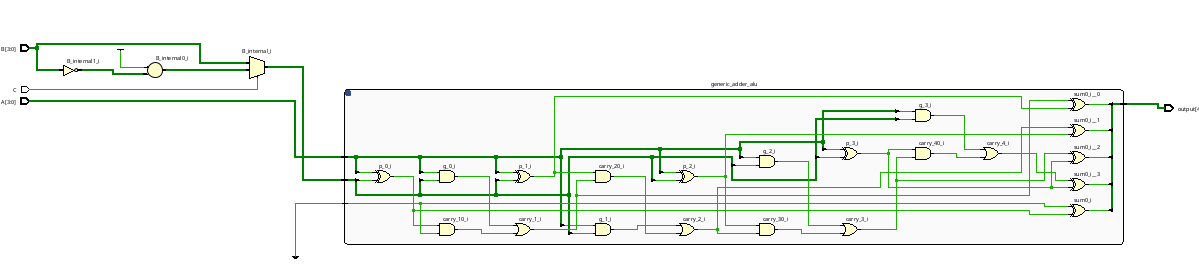
\includegraphics[width=1\textwidth]{assets/schematics/generic_4bit.png}
    \caption{Adder a 4 bit}
  \end{minipage}
    \begin{minipage}{0.45\textwidth}
    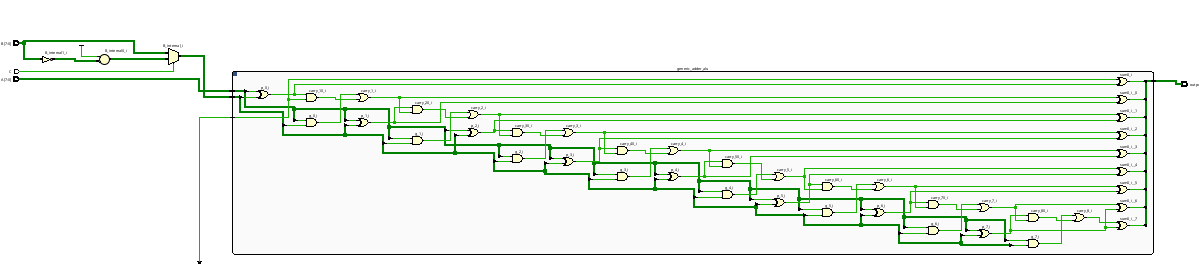
\includegraphics[width=1\textwidth]{assets/schematics/generic_8bit.png}
    \caption{Adder a 8 bit}
  \end{minipage}
    \begin{minipage}{1\textwidth}
    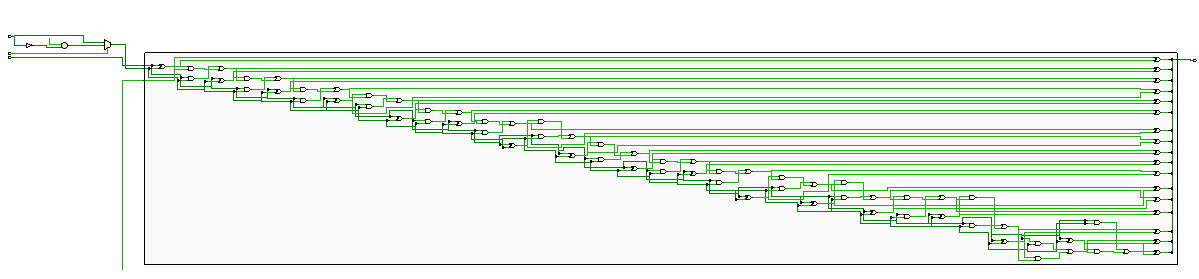
\includegraphics[width=1\textwidth]{assets/schematics/generic_16bit.png}
    \caption{Adder a 16 bit}
  \end{minipage}
\end{figure}
\newpage

\section{Mini ALU}
\subsection{Implementazione}
La mini ALU progettata presenta al suo interno un solo adder, preceduto da un multiplexer, che in base al bit di controllo C decide se dare in output B oppure il risultato di B invertito.
Nell'adder poi, oltre ad A ed al valore calcolato di B, verrà introdotto il valore di C stesso, completando il complemento a 2 in caso di necessità, non apportando cambiamenti altrimenti.

\begin{problem}{Codice Mini ALU}{}
\begin{lstlisting}[language=VHDL]
library IEEE;
use IEEE.STD_LOGIC_1164.ALL;

entity mini_alu is
  generic (bit_number : INTEGER := 4);
    Port ( A,B : in STD_LOGIC_VECTOR (bit_number-1 downto 0);
           C : in STD_LOGIC;
           output : out STD_LOGIC_VECTOR (bit_number downto 0));
end mini_alu;

architecture Behavioral of mini_alu is
  component generic_adder is
    generic (bit_number:INTEGER := 4);
      Port ( 
        A_adder, B_adder : in STD_LOGIC_VECTOR (bit_number-1 downto 0);
        cin : in STD_LOGIC;
        sum : out STD_LOGIC_VECTOR (bit_number downto 0));
  end component;

signal B_internal: STD_LOGIC_VECTOR (bit_number-1 downto 0);
signal carry_in: STD_LOGIC;

begin
      
  process(A, B, C) begin
    case C is
      when '0' => 
      B_internal <= B;
            
      when others =>
      B_internal <= STD_LOGIC_VECTOR(not B);

    end case;
  end process;

generic_adder_alu: generic_adder 
      GENERIC MAP (bit_number => bit_number)
      PORT MAP (
      A_adder => A,
      B_adder => B_internal,
      cin => C,
      sum => output);
end Behavioral;
\end{lstlisting}
\end{problem}

Possiamo trovare la schematica risultante nella \textit{Figure 4}
\begin{figure}[H]
    \centering
    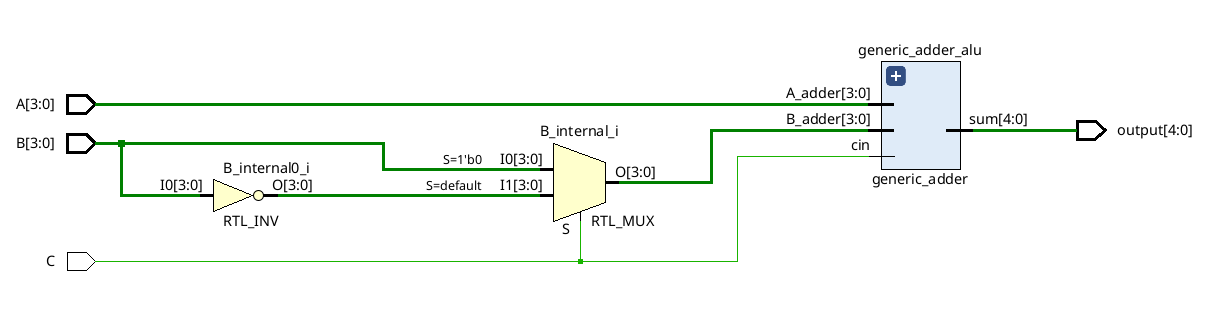
\includegraphics[width=15cm]{assets/schematics/generic_alu.png}
    \caption{Circuito Logico del mini ALU}
\end{figure}

\subsection{TestBench}
I test sono stati svolti in tutti i casi possibili, dando un tempo di 10 ns per ogni caso, con un tempo totale in nanosecondi: \begin{equation}2^{2n+1} \times 10\end{equation}

\begin{problem}{Codice test}{}
\begin{lstlisting}[language=VHDL]
library IEEE;
use IEEE.STD_LOGIC_1164.ALL;
use IEEE.NUMERIC_STD.all;

entity mini_alu_testbench is
    generic (n: integer := 4);
end mini_alu_testbench;

architecture Behavioral of mini_alu_testbench is
    component mini_alu is
    --generic (n : INTEGER := 4);
    Port ( A,B : in STD_LOGIC_VECTOR (n-1 downto 0);
           C : in STD_LOGIC;
           output : out STD_LOGIC_VECTOR (n downto 0));
    end component;
    
    constant min_value : integer := -(2**(n-1));
    constant max_value : integer := (2**(n-1))-1;

    signal Ia,Ib: STD_LOGIC_VECTOR (n-1 downto 0);
    signal Ic: STD_LOGIC;
    signal Ooutput: STD_LOGIC_VECTOR(n downto 0);
begin 
    CUT: mini_alu port map(Ia,Ib,Ic, Ooutput);
    process 
    begin
      external: for i in min_value to max_value loop
          Ia <= (STD_LOGIC_VECTOR((TO_SIGNED(i,n))));
          internal: for j in min_value to max_value loop
            Ic <= '0';
            Ib <= (STD_LOGIC_VECTOR((TO_SIGNED(j,n))));
            wait for 10ns;
            Ic <= '1';
            wait for 10ns;
         end loop internal;
       end loop external;   
    end process;
end Behavioral;
\end{lstlisting}
\end{problem}

\subsection{Simulazione}
Sono state effettuate simulazioni behavioural e post-implementation. Vediamole, evidenziandone le differenze.
\subsection{Behavioural}
\begin{figure}[h]
      \centering
      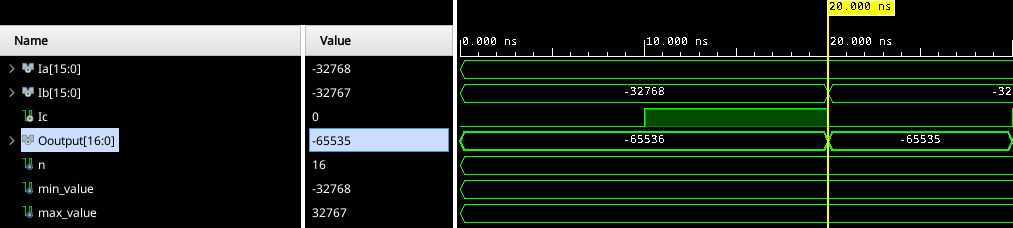
\includegraphics[width=1\textwidth]{assets/simulations/behavioural/16bit/end_first_ooutput_16bit_behav.png}
      \caption{Fine del primo input behavioural}
\end{figure}
\begin{figure}[h]
      \centering
      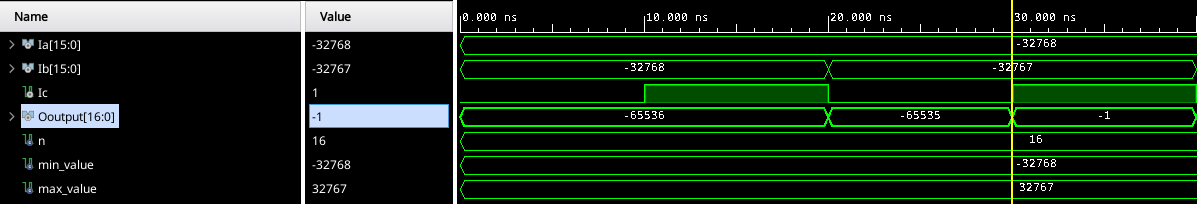
\includegraphics[width=1\textwidth]{assets/simulations/behavioural/16bit/start_secont_ooutput_16_bit_behav.png}
      \caption{Inizio del secondo input behavioural}
\end{figure}

\end{document}
